\subsection{Data Transfer Object}
\label{data-transfer-object}

\textbf{Scopo}: Comportamentale \\
\textbf{Raggio d'azione}: Oggetti

\paragraph{Definizione} Oggetti che trasportano dati tra processi per ridurre il numero di chiamate ai metodi

\paragraph{Applicabilità} È consigliabile utilizzare il pattern Data Transfer Object quando:
\begin{itemize}
    \item Si vogliono ridurre i viaggi di andata e ritorno al server raggruppando più parametri in un’unica chiamata;
\end{itemize}

\begin{figure}[H]
    \centering
    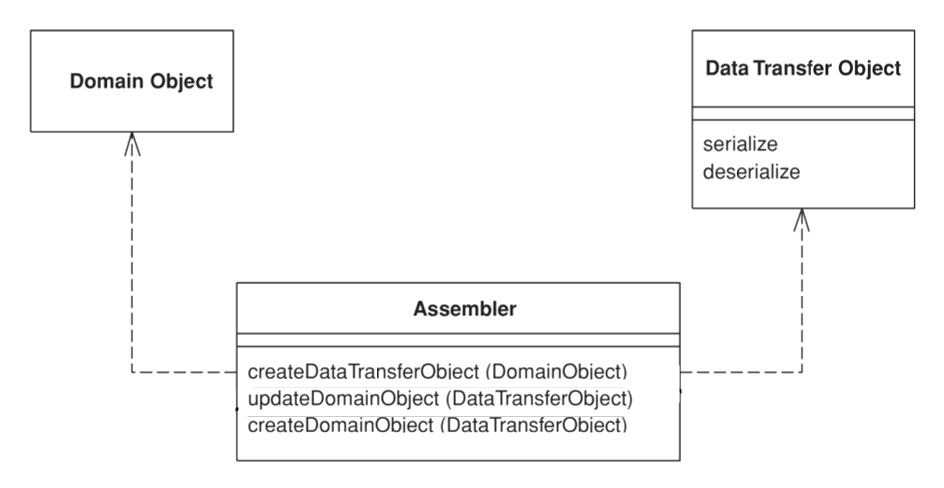
\includegraphics[width=0.75\linewidth]{assets/pattern/dto/dto-struttura.png}
    \caption{Class Diagram del pattern DTO}
\end{figure}

\paragraph{Struttura} I partecipanti del pattern sono:
\begin{itemize}
    \item \textbf{DomainObject}: Oggetto del dominio
    \item \textbf{DataTransferObject}: Oggetto da trasferire
    \item \textbf{Assembler}: Componente che realizza il mapping tra DO e DTO
\end{itemize}

\newpage